
As we have seen in Section \ref{solvingFEM}, the building of the elemental matrix and rhs
requires (at least) to assign a density and viscosity value to each quadrature point inside
the element. Depending on the type of modelling, this task can prove more complex than 
one might expect and have large consequences on the solution accuracy.

Here are several options:

\begin{itemize}
\item The simplest way (which is often used for benchmarks) consists in computing the 'real'
coordinates $(x_q,y_q,z_q)$ of a given quadrature point based on its reduced coordinates 
$(r_q,s_q,t_q)$, and passing these coordinates to a function which returns density and/or viscosity
at this location. For instance, for the Stokes sphere:
\begin{verbatim}
def rho(x,y):
    if (x-.5)**2+(y-0.5)**2<0.123**2:
       val=2.
    else:
       val=1.
    return val

def mu(x,y):
    if (x-.5)**2+(y-0.5)**2<0.123**2:
       val=1.e2
    else:
       val=1.
    return val
\end{verbatim}
This is very simple, but it has been shown to potentially be problematic. In essence, it can introduce very large contrasts inside a single element and perturb the quadrature. Please read section 3.3 of \cite{hedg17} and/or
have a look at the section titled "Averaging material properties" in the \aspect{} manual.

\item another similar approach consists in assigning a density and viscosity value to the nodes of the FE mesh first, and then using these nodal values to assign values to the quadrature points. Very often ,and quite logically, the basis functions are used to this effect. Indeed we have seen before that for any point $(r,s,t)$ inside an element we have
\[
f_h(r,s,t) = \sum_{i}^m f_i N_i(r,s,t)
\]  
where the $f_i$ are the nodal values and the $N_i$ the corresponding basis functions. 

In the case of linear elements ($Q_1$ basis functions), this is straightforward. In fact, the basis functions $N_i$ can be seen as moving weights: the closer the point is to a node, the higher the weight (basis function value). 

However, this is quite another story for quadratic elements ($Q_2$ basis functions). In order to illustrate the 
problem, let us consider a 1D problem. The basis functions are 
\[
N_1(r) =\frac{1}{2}r(r-1)
\quad\quad
N_2(r)=1-r^2
\quad\quad
N_3(r) =\frac{1}{2}r(r+1)
\]
Let us further assign: $\rho_1=\rho_2=0$ and $\rho_3=1$. Then 
\[
\rho_h(r) = \sum_{i}^m \rho_i N_i(r) = N_3(r)
\]  
There lies the core of the problem: the $N_3(r)$ basis function is negative for $r\in[-1,0]$. This means that the quadrature point in this interval will be assigned a negative density, which is nonsensical and numerically problematic!

{\color{red} use 2X Q1. write about it !}

\end{itemize}

The above methods work fine as long as the domain contains a single material. As soon as there are multiple fluids in the domain a special technique is needed to track either the fluids themselves or their interfaces. 
Let us start with markers. We are then confronted to the infernal trio (a {\it menage a trois}?)
which is present for each element, composed of its nodes, its markers and its quadrature points. 

Each marker carries the material information (density and viscosity). 
This information must ultimately be projected onto the quadrature points. Two main options are possible: an algorithm is designed and projects the marker-based fields onto the quadrature points directly or the marker fields are first projected onto the FE nodes and then onto the quadrature points using the techniques above.  

--------------------------




At a given time, every element $e$ contains $n^e$ markers. During the FE matrix building 
process, viscosity and density values are needed at the quadrature points. 
One therefore needs to project the values carried by the markers at these locations. 
Several approaches are currently in use in the community and the topic has been 
investigated 
by \cite{deka08} and \cite{dumg11} for instance.

{\sc elefant} adopts a simple approach: viscosity and density are considered to be elemental values, i.e. 
all the markers within a given element contribute to assign a unique constant density and viscosity 
value to the element by means of an averaging scheme. 

While it is common in the literature to treat the so-called arithmetic, geometric and harmonic means 
as separate averagings, I hereby wish to introduce the notion of generalised mean, which is a family 
of functions for aggregating sets of numbers that include as special cases the arithmetic, geometric and 
harmonic means. 

If $p$ is a non-zero real number, we can define the generalised mean (or power mean)
with exponent $p$ of the positive real numbers $a_1$, ... $a_n$ as:
\begin{equation}
M_p(a_1,...a_n)=
\left(
\frac{1}{n} \sum_{i=1}^n a_i^p
\right)^{1/p}
\end{equation}
and it is trivial to verify that we then have the special cases:
\begin{eqnarray}
M_{-\infty} &=& \lim_{p\rightarrow -\infty} M_p = \min (a_1,...a_n)                   \quad ({\rm minimum})  \\
M_{-1}      &=& \frac{n}{\frac{1}{a_1} + \frac{1}{a_2} + \cdots + \frac{1}{a_n}} \quad\quad  ({\rm harm.\; avrg.}) \\
M_{0}       &=& \lim_{p\rightarrow 0} M_p = \bigg(\prod_{i=1}^n a_i \bigg)^{1/n} \quad\quad  ({\rm geom.\; avrg.}) \\
M_{+1}      &=& \frac{1}{n}\sum_{i=1}^n a_i                                      \quad\quad\quad\quad\quad\quad  ({\rm arithm.\; avrg.}) \\
M_{+2}      &=& \sqrt{ \frac{1}{n} \sum_{i=1}^n a_i^2   }    \quad\quad\quad ({\rm root\;  mean \; square})  \\ 
M_{+\infty} &=& \lim_{p\rightarrow +\infty} M_p = \max (a_1,...a_n)     \quad ({\rm maximum}) 
\end{eqnarray}
Note that the proofs of the limit convergence are given in \cite{bull03}.  

An interesting property of the generalised mean is as follows:
for two real values $p$ and $q$, if $p<q$ then $M_p \leq M_q$.
This property has for instance been illustrated in Fig. 20 of \cite{scbe08}. 

One can then for instance look at the generalised mean of 
a randomly generated set of 1000 viscosity values within $10^{18}Pa.s$
and $10^{23}Pa.s$ for $-5\leq p\leq 5$. Results are shown 
in the figure hereunder and the arithmetic, geometric and 
harmonic values are indicated too. 
The function $M_p$ assumes an arctangent-like shape: very low values of p 
will ultimately yield the minimum viscosity in the array while very high values will 
yield its maximum. In between, the transition is smooth and occurs essentially for $|p|\leq 5$. 

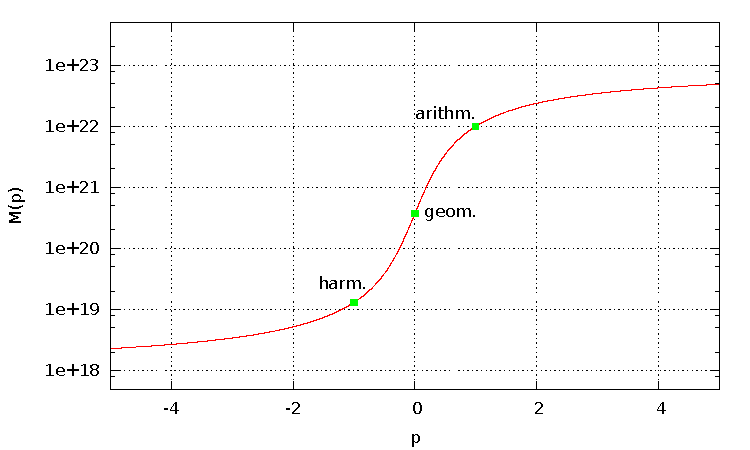
\includegraphics[width=12cm]{images/avrg/avrg.pdf}











\begin{mdframed}[backgroundcolor=green!5]
\begin{itemize}
\item[$\triangleright$] {\sl python\_codes/fieldstone\_markers\_avrg}
\end{itemize}
\end{mdframed}



